\documentclass[letter, 10pt]{article}
\usepackage{fullpage}
\usepackage[margin=0.5in]{geometry}
\usepackage{graphicx}
\usepackage{wrapfig}
\usepackage{caption}
\usepackage{subcaption}
\usepackage{listings}
\usepackage{hyperref}
\usepackage{amsmath}
\usepackage{float}

\pagenumbering{gobble}

\begin{document}
\noindent
\large \textbf{Rahul Ghosh} \hfill \textbf{Assignment\#2}\\
\normalsize Student ID: 5476965 \hfill CSci 5561\\

\section*{SCENE RECOGNITION}
\subsection*{Methods}
\subsubsection*{TINY IMAGE KNN CLASSIFICATION}
In this method each image is resized to a small fixed resolution to get a tiny image representation. This tiny image is transformed to a vector and normalized to get a zero mean and unit length vector. KNN classification is used on the vectorized data. The accuacy obtained is 23.8667 and the confusion matrix is shown in 


\subsection*{Results}

\begin{figure}[h]
    \minipage{0.33\textwidth}
        \centering
        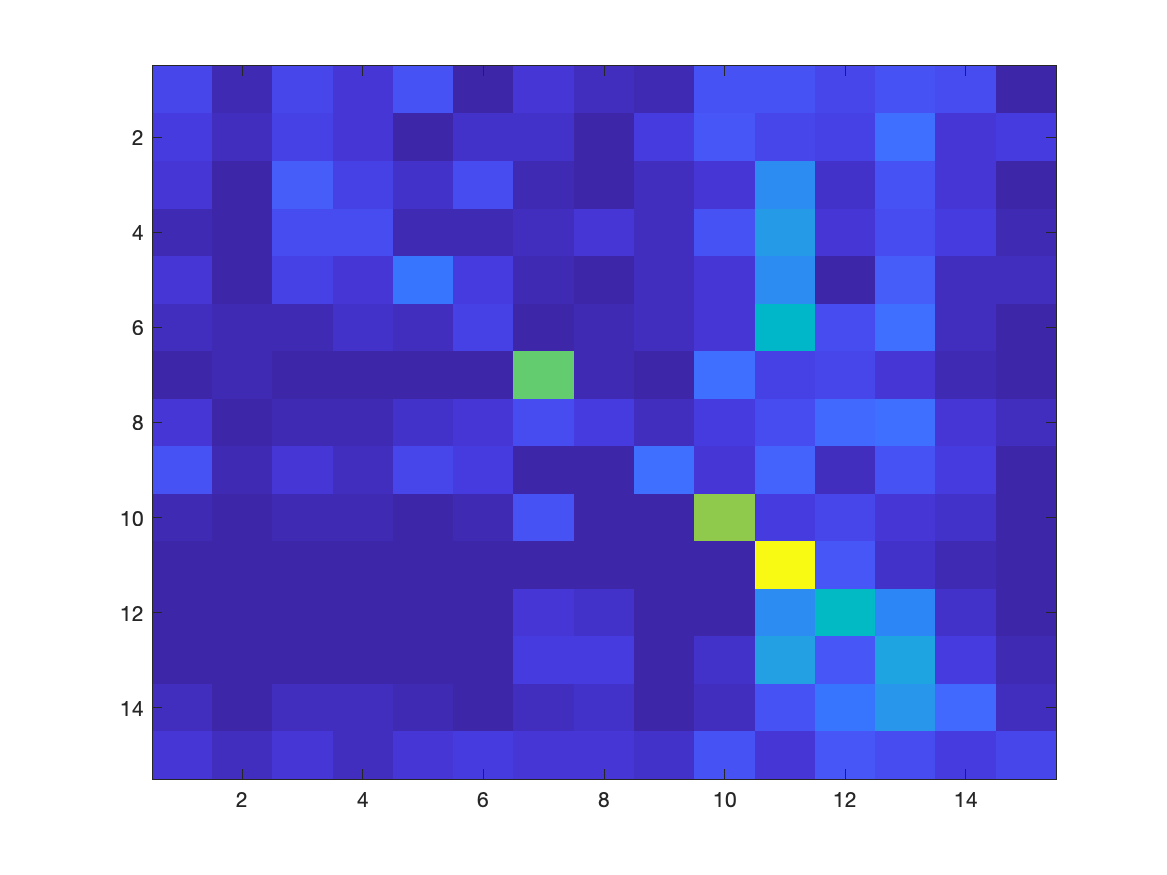
\includegraphics[width=\textwidth]{HW3/RESULT/ClassifyKNN_Tiny_confusion.png}
        \subcaption{Confusion matrix for Tiny-KNN}
    \endminipage\hfill
    \minipage{0.33\textwidth}
        \centering
        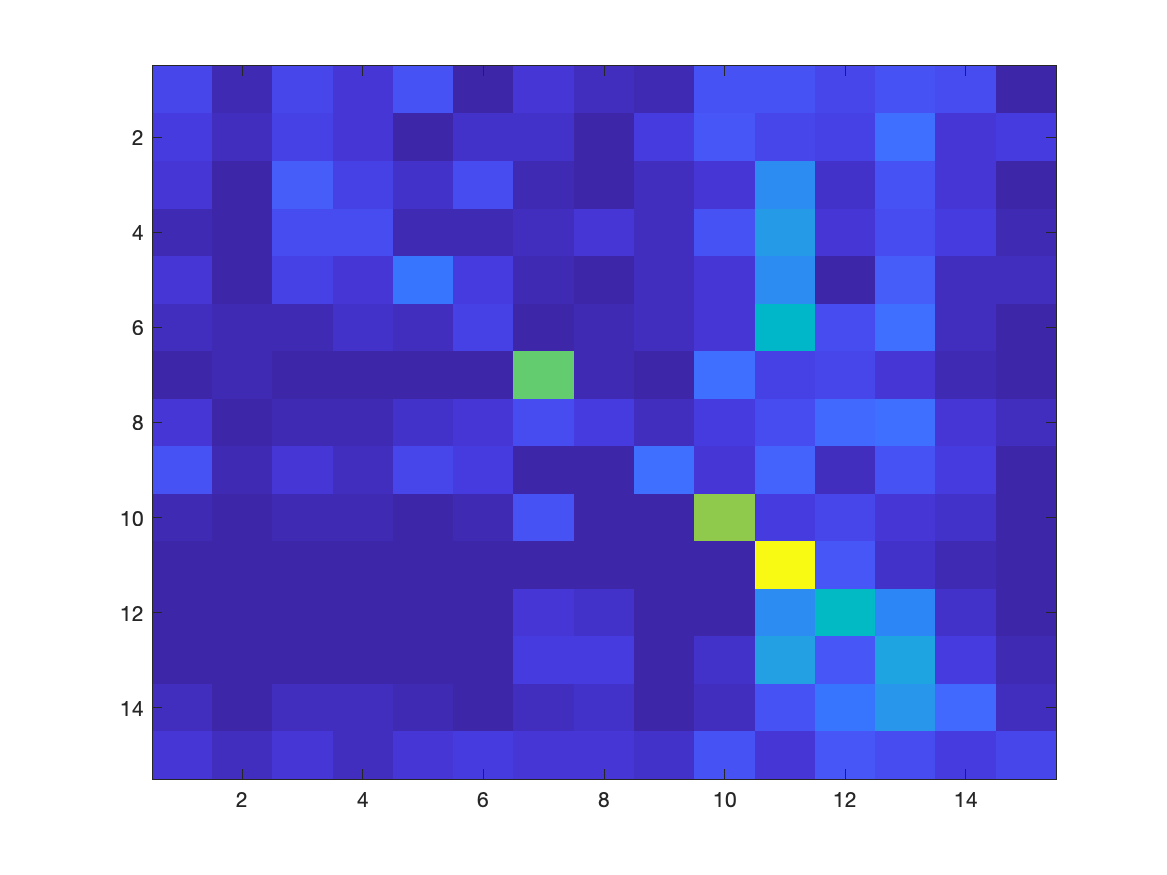
\includegraphics[width=\textwidth]{HW3/RESULT/ClassifyKNN_Tiny_confusion.png}
        \subcaption{Confusion matrix for BoW+KNN}
    \endminipage\hfill
    \minipage{0.33\textwidth}
        \centering
        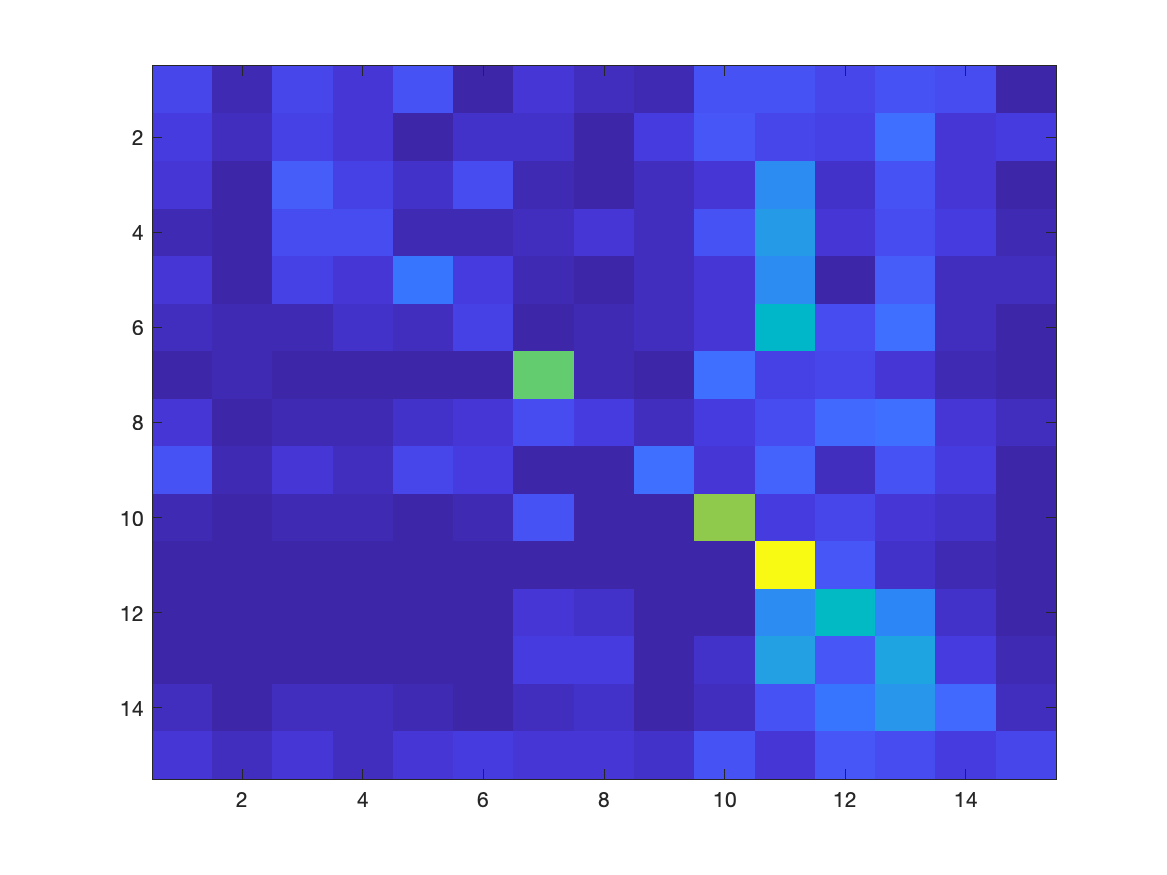
\includegraphics[width=\textwidth]{HW3/RESULT/ClassifyKNN_Tiny_confusion.png}
        \subcaption{Confusion matrix for BoW+SVM}
    \endminipage\hfill
\end{figure}

\end{document}